\documentclass[UTF8,AutoFakeBold,scheme=chinese,eversion]{GXMU-Thesis}
\usepackage{amsmath,amsthm,amssymb,amsfonts}
\definecolor{nuanbai}{HTML}{F5F5F5}
\pagecolor{nuanbai!5}
% 浮动环境设置
% 默认情况下, \LaTeX{} 要求每页的文字至少占据 20%,否则该页就只单独放置一个浮动环境,
% 而这通常不是我们想要的, 我们将这个要求降低到 5%.
\renewcommand*{\textfraction}{0.05}
% 有时如果多个浮动环境连续放在一起,
% 会将它们分在几个不同页,即使它们可在同一页放
% 得下. 我们可以通过修改 |\topfraction| 和 |\bottomfraction| 分别设置顶端和底端的浮
% 动环境的最大比例.
\renewcommand*{\topfraction}{0.9}
\renewcommand*{\bottomfraction}{0.8}
% 有时\LaTeX{}会把一个浮动环境单独放在一页,
% 我们要求这个环境至少要占据 85% 才能单独放在一页.
% 注意:  |\floatpagefraction| 的数值必须小于 |\topfraction|.
\renewcommand*{\floatpagefraction}{0.85}
% 关于图片 graphicx
% 如果图片没有指定后缀, 依次按下列顺序搜索
\DeclareGraphicsExtensions{.pdf,.eps,.jpg,.png}
% 设置图表搜索路径, 可以给图表文件夹取如下名字
\graphicspath{{figures/}{figure/}{pictures/}{picture/}{pic/}{pics/}{image/}{images/}}
\usepackage[physics]{stys/physicx}
\usepackage{stys/Symbols}
\usepackage{amsfonts}
\usepackage{mathrsfs}
\usepackage{enumitem}
\setlist{nosep,font=\upshape} % 取消所有列表默认距离

\setlength{\headheight}{14.45398pt}
\usepackage{appendix}
\usepackage[sort&compress]{gbt7714}
\citestyle{numbers}% 可选参数含义:存在多篇引文时自动压缩序号
\usepackage{bropd}
\begin{document}
\author{陆世龙}
\teacher{卢卫君教授}
\subject{基础数学}
\major{复代数几何}
\academy{数学与物理学院}
\finishedtime{2022年9月}
\grade{2022级}
\subtitle{微分几何中的相关问题研究与说明}
\logo{minda-removebg.png}
\makecover
{\renewcommand\headrulewidth{0pt}
\fancyhead[C]{}

\thispagestyle{empty}
{\centering
{\large 分类号:\uline{O175.29}\hspace{1.5cm}密级:\uline{公开}\\[2cm]
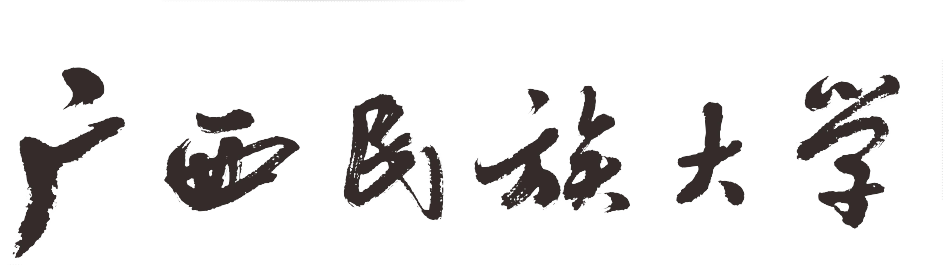
\includegraphics[width=.45\linewidth]{mdn-removebg.png}}\\[1.5cm]
\hspace*{2em}\makebox[.7\linewidth][s]{\huge 硕士研究生学位论文}\\[1.5cm]
\makeatletter
{\fontsize{15.75pt}{15.75pt}\selectfont\bfseries\@subtitle}


\vfill

{\large
\begin{center}
\begin{tabular}{lcc}
        \makebox[.22\linewidth][s]{学位类别}&: & \makebox[.25\linewidth][s]{ 理学硕士} \\[-5pt]\cmidrule[0.85pt]{3-3}
        \makebox[.22\linewidth][s]{学科专业} &:& \makebox[.25\linewidth][s]{\@subject} \\[-5pt]\cmidrule[0.85pt]{3-3}
        \makebox[.22\linewidth][s]{研究方向} &:& \makebox[.25\linewidth][s]{\@major} \\[-5pt]\cmidrule[0.85pt]{3-3}
        \makebox[.22\linewidth][s]{研究生} &:&\makebox[.1\linewidth][s]{\@author} \\[-5pt]\cmidrule[0.85pt]{3-3}
        \makebox[.22\linewidth][s]{指导教师} &:&\makebox[.2\linewidth][s]{\@teacher} \\[-5pt]\cmidrule[0.85pt]{3-3}
\end{tabular}
\end{center}}
\makeatother


\bigskip

\vfill
\hfill 论文完成时间: \hspace{1.5em}年\hspace{1.5em}月\hspace{1.5em}日
}
\clearpage
\originalitydeclaration % 独创性声明
\pagenumbering{Roman}
\begin{center}
    {\fontsize{20}{20}\selectfont\bf 微分几何学问题的探究与讨论研究}
\end{center}
\vspace{.2cm}
\begin{cnabstract}
\vspace*{.2cm}
    这是摘要模拟. 
    
    本人已经认真阅读某某的“研究生学位论文著作权管理规定”, 同意本人所撰写学位论文的使用授权遵照学校的管理规定:  学校作为申请学位的条件之一, 学位论文著作权拥有者须授权所在大学拥有学位论文的部分使用权, 即:
    
    已获学位的研究生必须按学校规定提交印刷版和电子版学位论文, 学校可以采用影印、缩印或其他复制手段保存研究生上交的学位论文; 为教学和科研目的, 学校可以将公开的学位论文或解密后的学位论文作为资料在图书馆、资料室等场所或在校园网上供校内师生阅读、浏览. \\[.5em]
   
    \chinesekeyword{义逆 ; 广义奇异值分析 ; 偏序集 ; 核心-幂零分解 ; 模糊正则矩阵}
\end{cnabstract}














\clearpage
% \thispagestyle{empty}
\begin{center}
    {\fontsize{16}{16}\selectfont\textbf{\MakeUppercase{ Monotone Iteration Methods For Some Generalized Hifer Fractional Differential Equations}}}
\end{center}
\vspace{.2cm}
\begin{enabstract}
\vspace*{.2cm}
Several approaches have been proposed for estimating the glass transition temperature of mixtures and random copolymers from knowledge of the properties of the pure components. Although different in detail, the proposed relationships are all based on the additivity of basic thermophysical properties. One of the most popular equations for predicting glass transition temperatures of amorphous mixtures and random copolymers is the Gordon-Taylor equation:\\[.5em]

\englishkeyword{Monotone iteration method: Generalized fractional deriverted}
\end{enabstract}


\clearpage
}
\thesisfigurelist                                                      % 插图目录
\thesistablelist                                                     % 插表目录                                  
\tableofcontents\clearpage  

\pagenumbering{arabic}
\section{什么是复几何?}

\subsection{复流形 Complex Manifolds}
要了解复几何, 我们首先需要掌握复流形的基本概念\cite{Fujihechubujiqiwuliyingyong}. 

映射 $f: \mathbb{C}^m \rightarrow \mathbb{C}^n:\left(z^1, \cdots, z^m\right) \mapsto\left(w^1, \cdots, w^n\right)$ 是全纯的. 如果对于每个 $w^i$ 都是 $z^j$ 的全纯函数.  $(1 \leq i \leq n, 1 \leq j \leq m)$. 存在着一种特殊的拓扑空间 $M$ 有着一族开覆盖 $\mathcal{U}$, 如果对于开覆盖当中的任何子集 $U$ ,  存在着同态映射 $\phi_U: U \rightarrow \mathbb{C}^n$ 使得对开覆盖中的任何两个相交子集 $U ,  V$  ,  转 移 函 数 $ \phi_{U V}:=\phi_U \phi_V^{-1}$ 是全纯的,  则称拓扑空间为复流形 $M$ . 

常见的复流形有 Grassmannian 流形 $G_{k, n}(\mathbb{C}) ,  k$ 维复向量空间的子空间, 最常见的例子 $G_{1, n}=\mathbb{C} P^n , $ Flag 流形是一类在研究Penrose--Ward correspondence 所使用的重要流形. 

若$L_1 \subset \cdots \subset L_r \subset \mathbb{C}^n, \quad \operatorname{dim}_{\mathbb{C}} L_i=d_i$, 则 $\left(L_1, \ldots L_r\right)$ 称为 $\mathbb{C}^n$ 当中的 Flag, Flag 流形 $F_{d_1, \ldots, d_r, n}$ 定义为 

\[F_{d_1 \cdots d_r}:=\left\{ \text{all flags }\left(L_1, \ldots, L_r\right)\text{ with }\operatorname{dim}_{\mathbb{C}} L_i=d_i, i=1, \ldots r\right\},\]
也可以写成
\begin{align*}
F_{d_1 \ldots d_r, n}=\frac{U(n)}{U\left(n-d_r\right) \times \cdots \times U\left(d_2-d_1\right) \times U\left(d_1\right)} \text {, }
\end{align*}
很容易可以求出维数. 除此之外还有 Stein 流形, 能够嵌入复欧式空间的子流形, 在 $\check{C} e c h$ 上同调中有重要应用. 
单单只有流形末免过于枯燥, 我们要在流形上定义一些运算. 给定一个实向量空间, 定义映射 $I: V \rightarrow V$ , 并且有 $I^2=-1_V$ 称为向量场的复结构, 这要求实向量场是偶数维的. 以一种显然的复结构被称为正则复结构:
\[I: \mathbb{R}^{2 n} \rightarrow \mathbb{R}^{2 n}, I\left(x^1, \ldots x^n, y^1, \ldots, y^n\right)=\left(-y^1, \ldots,-y^n, x^1, \ldots, x^n\right)\]
给定一个偶数维的实可微流形 $M$ , 流形上的 $(1,1)$ 形光滑张量场 $I$ 称为近复结构, 原因是对于流形每一个点上的切空 间 $T_x M$ 都存在着复结构 $I_x$ , 装备了张量场 $I$ 的流形称为近复流形. 

考虑切空间的的复化 $T M^C=T M \otimes_{\mathbb{R}} \mathbb{C}$ , 每个点的复化切空间可以分解为两个子空间分别是复结构 $I$ 关于特征值 $\pm i$ 的特征子空间, 分别记作 $T^{1,0} M, T^{0,1} M$ , 切丛和余切丛的截面分别是 $(1,0)$ 型和 $(0,1)$ 型的向量场, 又叫做全 纯和反全纯的切丛. 与复切空间类似可以通过对实流形上微分形式的复化得到复流形 $M$ 上的复微分形式
$\Omega^q(M)^c:=\Omega^q(M) \otimes_{\mathbb{R}} \mathbb{C}$, 根据 $\omega\left(V_1, \ldots, V_n\right)=0$ 当中 $V_i$ 分别属于 $T^{0,1} M, T^{1,0} M$ 的个数是 $s, r$ . 可以将 微分形式写成 $\Omega^{r, s}(M)$,整个余切丛可以表示为直和 $\oplus_{r+s=q} \Omega^{r, s}(M)$ . 显然 $\Omega^{1,0}(M)$, $\Omega^{0,1}(M)$ 当中的元素和 $T^{1,0}(M), T^{0,1}(M)$ 的元素对偶. 这一点从正交关系 $<d z^i, \frac{\partial}{\partial \bar{z}^j}>=0,<d z^i, \frac{\partial}{\partial \bar{z}^j}>=\delta_j^i$ 等可以看出. 

在切丛和余切丛的截面上可以定义一些其他运算, 其中比较的典型的运算就是张量积和外微分这两种运算. 给定一个微 分形式
\begin{align*}
\omega=\frac{1}{r ! s !} \omega_{i_1 \ldots i_r \bar{i}_{r+1} \ldots \bar{i}_{r+s}} d z^i \wedge \cdots \wedge d \bar{z}^{i_r+s}
\end{align*}

外微分算子作用上该微分形式上成为
\[d \omega=\frac{1}{r ! s !}\br{\partial_k \omega_{i_1 \ldots \bar{i}^{r+s}} d z^k \wedge d z^{i_1} \wedge \ldots d \bar{z}^{i_r+s}+\bar{\partial}_{\bar{k}} \omega_{i_1 \ldots \bar{i}_{r+s}} d z^{i_1} \wedge \ldots d \bar{z}^{\bar{k}} \wedge \ldots d \bar{z}^{\bar{i}_r+s} },\]
其中 $\partial: \Omega^{r, s}(M) \rightarrow \Omega^{r+1, s}(M) , \bar{\partial}: \Omega^{r, s}(M) \rightarrow \Omega^{r, s+1}(M)$, 这两个算符又被称为 Dolbeault 算子, 与 deRham 上同调当中的微分算子 $d$ 有类似的性质 $\partial^2=\bar{\partial}^2=0$ , 从而可以构造 Dolbeault 上同调群. 
接着研究一种流形上一种的特殊的结构, 称为 Hermitian 结构. 给定一个复向量空间 $(V, I)$ , 定义一种双线性映射 $h: V \times V \rightarrow \mathbb{C}$, 满足 :
\begin{enumerate}[label=(\roman*)]
    \item 对于任何 $u, v \in V, h(u, v)$ 是 $\mathbb{C}$-线性的,
    \item $\bar{h}(u, v)=h(v, u)$,
    \item $h(u, u) \geq 0$ , 当且仅当 $u=0$ 时取等.
\end{enumerate}
当我们企图通过近复结构将光滑实流形看成复流形的时候, 可以将原有流形上的黎曼度量推广成 Hermite 度量, 即 $g_x: T_x M^C \times T_x M^C \rightarrow \mathbb{C}$ , 并且满足
$g_x(X+i Y, U+i V) \rightarrow g_x(X, U)-g_x(Y, V)+i\left(g_x(X, Y)+g_y(Y, U)\right)$, 并且满足
$g_x\left(I_x X, I_x Y\right)=g_x(X, Y)$ 称为 Hemitian 度量. 给定 $T^{1,0}(M), T^{0,1}(M)$ 上的基 $\left(\frac{\partial}{\partial z^i}\right),\left(\frac{\partial}{\partial \bar{z}^i}\right)$, 求得 Hermitian 度量的具体形式 $g=g_{i \bar{j}} d z^i \otimes d \bar{z}^{\bar{j}}+g_{\bar{i} j} d \bar{z}^{\bar{i}} \otimes d z^j$ . 

具有 Hermite 度量的流形称为 Hermite 流形, 记作 $(M, g)$ , 对于一个给定的 Hermite 流形 $(M, g)$ , 定义一个 $(1,1)$ 型张量场 $J(X, Y)=g(I X, Y)$ , 容易验证该张量场是反对称的, 即 $J(X, Y)=-J(Y, X)$ , 称为 K\"ahler 形式. 
K\"ahler 流形作为一类重要的流形, 有如下三种等价定义:
\begin{enumerate}[label=(\roman*)]
    \item $d J=0$,
    \item $\nabla J=0$,
    \item $\nabla I=0$.
\end{enumerate}
其中 $\nabla$ 是 $g$ 的 Levi-Civita 联络, 根据 Kähler 流形上度量的特殊性质, 可以诱导出挠率和曲率的特殊性质.  (挠率和曲率的定义与黎曼几何一致) Riemann 和 Ricci 张量可以被简化为 $R_{i \bar{j} k \bar{l}}=g^{i \bar{s}} \frac{\partial \Gamma_{\bar{j} \bar{l}}^{\bar{s}}}{\partial z^k} , \textrm{Ric}_{_{\bar{i} j}}:=R^{\bar{k}}{ }_{i \bar{k} j}$ ,由 Ricci 张量可以诱导出对应的 Ricci form: $\mathscr{R}(X, Y):=\operatorname{Ric}(I X, Y)$ , Ricci form 为 0 , 称之为是Ricci平坦的, Ricci平坦的 K\"ahler流形是 Calabi-Yau 流形. 而在弦理论里面场的概念可以定义为从黎曼面 (一维复流形) 到 Calabi-Yau 流形的一种特殊映射. 

\section{复几何的研究方向有哪些?}

\subsection{复几何的具体研究方向及其当今进展}
\subsubsection{代数曲线}
代数曲线论近期的一个重要进展就是经典问题 Brill-Noether 猜想的解决, 这是由 Gri ffiths 和 Harris 解决的. 该问题是 关于一般曲线上给定次数和维数的线性系的集合的维数的计算, 可以认为现在对一般曲线的情形已经有了足够的认识, 然 而还留下几个问题, 比如一般公设性, 即给定射影空间中一条足够一般的曲线, 先验地确定具有给定的次数, 而且包含这 条曲线的超曲面的个数. 又如 $\mathbb{P}^3$ 或更一般的 $\mathbb{P}^n$ 中曲线的研究已经取得了进展, 即目前已知一条这样的曲线所有可能的
甚至平面的曲线的情形也没有得到很好的理解, 关于 Severi 的给定次数且具体确定个数的二重点的不可约平面曲线簇的 不可约性的断言一直末能证明, 然而这个断言有一个著名的推论—Z Zariski 猜想, 即 $\mathbb{P}^2-C$ 的基本群是交换群, 其中 $C$ 是一条具有通常二重点的平面曲线, 这个却已被 Fulton 和 Deligne 直接证明.

亏格为 $g$ 的代数曲线的同构类的集合构成一个 $3 g-3$ 维代数簇一一参量空间(l'espac e des Modulus) $M_g$ , 除了小的 $g$ 以外这方面的研究甚少. Harris 和 Mumford 还给出了一个著名的论断, 即 $g \geq 24$ 时 $M_g$ 是一般概形, 特别地这里 蕴含一条亏格为 $g$ 的一般曲线不能用 $3 g-3$ 个独立的参量来描述. 参量空间 $M_g$ 的拓扑提出了一些有趣的难题, 利用 Thurston 的方法, Harer 和 Miller 已经做出了一些振奋人心的结果, 但在这个领域中还有许多问题待解决.

\subsubsection{曲线和 Abel 簇, \texorpdfstring{$\theta$}  函数}
近期的一项重大突破就是发现了产生于物理的一些非线性方程(如 Korteweg-De Vri es 方程和 Toda 格等) 与代数曲线及 其 Jacobi i簇的几何之间的深刻联系, 这样就使得某些微分算子代数与一条代数曲线的几何之间的对应 ( Kriěever 词典),  从而能借助 $\theta$ 函数型的函数显式地解方程. 在上述所考虑的方程中, 某些簇(如 KdV 系统和 KP 系统)具有对称性, 且在仿 射 Lie 代数中可以得到解释. 其它的方程则来自经典力学, 特别是完全可积的 Hamilton 系统理论, 于是就可以归结为这 些系统在 Abel 簇上的积分, 这些簇可作为 Jacobi 簇或 Prym 簇被显式描述, 因此是一个蓬勃发展的邻域, 它与数学物 理的其它分支有很强的联系 .

上面的结果都被应用于解决一个经典问题——Schottky 问题, 即在所有 Abel 簇中如何刻画曲线的 Jacobi 簇.

Novikov 曾猜测当 $\theta$ 函数满足 $K P$ 第一方程足以刻画 Jacobi 簇, 这个猜测可能过于乐观, 但已经得到了引人注目的部 分结果, 事实上 Schottky 问题的经典方法俑过 $\theta$ 函数零点的多项式方程来刻画 Jacobi 簇近期也有进展.
\subsubsection{曲面}
自从意大利学派提出了代数曲面的一个分类后, 日本数学家 Kodaira 又把它推广到了紧复曲面, 这表明可以通过典范系 和多重典范系的性质能够分出一些特殊类型的曲面, 并且能够精确地描述它们(如有理曲面和 $K 3$ 曲面等) , 当然还剩下一 个几乎囊括一切的大类―一般型曲面 .

一般型曲面在近十年内得到了广泛的研究, 即对多重典范映射的性质和数值不变量之间的关系已经有了足够的了解. 但这 些曲面的集合目前就好比一个没有显著结构的标本库, 数学家们已经构造和研究了大量的例子, 却没有看到具有普遍意义 的现象出现, 这说明在这个领域还缺少一个具有指导性的思想.

特殊型曲面, 尤其是 $K 3$ 曲面和 Enriques 曲面, 借助关于周期的深刻结果已经得到了广泛的研究, 这些曲面的几何(包 括自同构和嵌入等现在已经被广泛认识, 但参量空间的情况却有所不同, 它的结构衍生出了一些有趣的问题, Gieseker 给出了对一般型曲面参量空间是存在的, 但对于其几何的研究却是一片空白.

日本学派对开曲面的研究十分有兴趣且得到了非常类似于紧的情形的分类, 这里提一下 Kodaira 分类在还有一个情形 $\longrightarrow \mathrm{VII}_0$ 型曲面, 对它的描述近年来已取得了进展, 然而也遇到了许多问题 .
\subsubsection{维数 \texorpdfstring{$\geq 3$}  的簇}

曲面的分类对任意维数而言有一个自然推广, 其重要的工具就是 Kodaira 维数不变量, 它与多重典范系的性质有关.一个 簇如果被称为是一般型, 那么它满足 Kodaira 维数等于其维数, 否则这个簇就属于特殊型. 日本学派对簇的类型进行了研 究, 在研究过程中 $C_{m, n}$ 和 $C_{m, n}^{+}$猜想起着重要的作用, Kawamata 和 Viehweg 对好几种情形均给出了证明, 由此得出 了维数 $\geq 3$ 的簇的分类轮廓, 但尚有许多问题有待解决.

$3$ 维簇的双有理几何比曲面要复杂得多, 特别地当还不清楚极小模型的等价概念是, 但由于 Mori 的工作, 沿着这个方向 已经跨出了坚实的一步, 让我们有希望得到极小模型的存在性, 只要允许某些简单奇点的存在性, 即 Mori 已经证明了 3 维簇极小模型的存在性. 另外两个问题 (关于典范环的有限生成性和双有理态射的分解问题) 与上述的问题有联系, 近期也 取得了重大进展, 其中 3 维情形的典范环的有限生成问题已经解决. 以上这些问题都是十分有趣的问题并具有很强的生 命力, 尽管离完全解决还有一段距离.

最后提一下由 Iskovskih 和 Mori-Mukai 作出的 Fano 簇 (即负典范除子为丰沛的 3 维簇) 的完全分类以及 Iskovskih 对 某些 Fano 簇的双有理自同构群的研究, 后一个研究提供了一个关于 Fano 簇的非有理性的判别法, 另一个判别法则是借 助中间 Jacobi 簇. 总之可以认为有理性问题在 3 维情形时已经初步得到解决, 但在更高维的情形则没能取得突破.

\subsubsection{向量丛}

代数向量从在近几年里已经被广泛的研究,主要是对射影空间 $\mathbb{P}^n$ 上的向量从已经得到了各种结果,尤其是 $n$ 比较小和 秩也有了一般的方法如跳跃直线和 monade) . 至于参量空间的一个有趣的问题现在已经有了结果 .
这些问题的强大动力大多来自它与规范场的物理理论的惊人联系,如 $S_4$ 上 Yang-Mills 方程的解可由 $\mathbb{P}^3$ 上某些秩 2 向 量从(称为瞬子)所提供,目前已经能部分地描述这些向量从的参量空间,但还不清楚对于取定次数的向量从是否不可约.
另一个有趣的问题是当 $n \geq 5$ 时 $\mathbb{P}^n$ 上秩 2 的不可分解向量从的存在性问题,它与下面的问题有密切联系,即当 $n \geq 6$ 时 $\mathbb{P}^n$ 中的一个余维数为 2 的簇是否为两个超曲面的交,尽管 Zak 作出了漂亮的结果,但这个问题仍无法解决.
\subsubsection{计算几何}

这个经典几何的分支是寻求计算,如与 5 个给定的圆锥曲线相切的平面圆锥曲线的个数,或与一条空间曲线交于 4 个点 的割线条数 . 当然重点不在于结果本身,而是在于得到这些结果的技巧 .

上面所说的技巧之一就是相交理论,它是在适当的 Chow 环中设法定义两个子簇的相交闭链. 当环绕簇为非奇异簇时,就 可以直接使用相交理论,而在一般情形下 Fulton 的工作提供了一个满意回答,从而使得很多计数问题能被解决,一个引 人注目的应用就是通过 Chern 类的某些多项式的正性来刻画向量从的丰沛性 .

计数几何的另一经典内容就是完全簇空间的定义. 这个问题在某些低次数的情形有了一些结果,而一般情形则是十分复杂 的. 其它的一些问题,比如一个射影簇的多重割线的条数计算或一个浸入的重点数的计算,实际上就是对某些几何地定义 的簇的特征类的表示,关于这些问题已获得了很多结果,似乎数学家们已有了相当清楚的了解.
\subsubsection{Hodge 理论}

非奇异复射影簇 $X$ 的上同调具有一个 Hodge 结构 ,就是一个分解 $$H^n(X, C)=\bigoplus_{p+q=n} H^{p, q}$$ 且满足 $H^{q, p}=\overline{H^{p, q}}$.

Torelli 问题就是给定 Hodge 结构(这等价于给定 $X$ 上 $n$-形式的周期矩阵)是否足以决定一个簇. 这是一个困难而又引人 人胜的问题,目前还仅仅知道在几种特殊情况下的答案,即曲线,某些 3 维簇和 $K 3$ 曲面,这里的最后一个情形现在已 完全搞清楚了,其结果格外引人注目,即给出一个曲面等价于给出其 Hodge 结构,这样一来对于 $K 3$ 曲面的参量空间有 了一个非常确切的超越描述.

Griffiths 及其学派用不同的方法研究 Torelli 问题 , 他们不是从单独的 Hodge 结构 , 而是从它的无穷小形变来重新构造簇. 事实表明这种方法提供了较易处理的几何对象,这个方法使得对几乎所有的超曲面都能证明一般的 Torelli 定理.
周期映射(即使一个簇与其 Hodge 结构相伴)的研究提出了许多其它问题,它成为个非常有趣的课题.

开簇或奇异簇允许带有混合 Hodge 结构,这是通常 Hodge 结构的扩展. 尽管是关于奇点的内容,但必须指出奇异簇的 混合 Hodge 结构在退化的研究中起着重要的作用. 另一方面 $\mathscr{D}$-模理论的一个主要问题之一就是在奇异簇的相交上同调 上定义一个纯 Hodge 结构 .
\subsubsection{代数闭链}

尽管代数簇上余维数为 1 的闭链一一除子的群结构是相当清楚的, 但余维数 $\geq 2$ 时却并非如此. 数学家们在这个群上给 出了一些等价关系,包括有理等价,代数等价和同调等价. 对非奇异代数簇上闭链的群关于上述等价关系的商群的㓈究是 代数几何的一个主要问题.
闭链群关于有理等价的商群称为 Chow 群. Chow 群一般是很大的,甚至大到不能成为代数群,对 0 -闭链的情形,
Roitman 和 Bloch 使上述断言精确化了,相反地他们证明了挠子群是具有有理大小的,要指出的是甚至对于某些曲面还 不知道 0 -闭链的 Chow 群是零还是非常大.

代数 $K$-理论给出了 Chow 群的方法并提供了一个上同调解释. 这个方法尽管使用起来并不总是容易的,但是能得到某些 结果,特别是关于 0 -闭链和余维数为 2 的闭链的结果.

关于闭链的代数等价则知道得极少.一般来说它与同调等价不一般,更糟的是 Cleme -ns 发现同调平凡的闭链所成的群模 去代数等价之后可能不是有限型的,故这个群仍是很神秘的.

Hodge 理论为闭链的研究提供了一个重要工具—一中间 Jacobi簇 . 这个复环面对于闭链所起的作用就像曲线的 Jacobi 簇对其除子所起的作用一样,但相应的阐述就更困难 . Griffiths 的作为解决 Hodge 猜想可能的途径而引入的正规函数方 法显示出非常丰富的内容,尽管对其原始目的不太有效 . 代数闭链和 Hodge 结构之间的关系构成了一个困难但又是基础 的课题,这个课题在今后几年内将会有所进展.

最后提一下 Hodge 猜想,这个猜想把代数闭链的上同调类刻画为 Hodge 分解的 $(p, p)$ -型有理类,目前这个基本猜想 毫无进展 . 尽管如此还是应该引述 Deligne 的一个结果,尽管这个结果是算术性质的,即数域 $K$ 上Abel 簇 $(p, p)$-型类 的概念有一个内在的含义, 与 $K$ 在 $C$ 中的嵌入无关.\cite{DaishujiheGeometrieAlgebrique}

以上就是关于我的研究方向的简要陈述.







\newpage
{
\thispagestyle{bibstyle}
\bibliographystyle{gbt7714-numerical}   % 我选择了使用顺序编码制
\bibliography{ref}
}
\thesisacknowledgement                                                 % 致谢
\thesisaccomplish                                                      % 攻读专业硕士学位期间取得的成果
\end{document}
